\textbf{Chapter 2: Underlying Concepts}

\begin{center}
    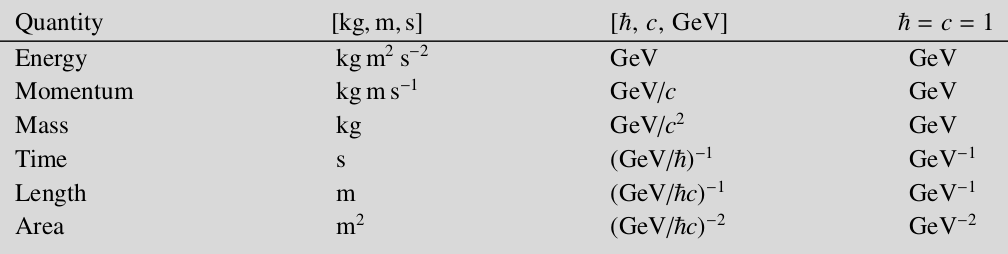
\includegraphics[width=\linewidth]{images/natural_units.png}
\end{center}


\begin{multicols}{2}
    Sig. $(1, -1, -1, -1)$
    \begin{align*}
        \gamma &= \frac{1}{\sqrt{1 - \frac{v^2}{c^2}}}\\
        d' &= d/\gamma\\
        E^2 &= \vec{p}^2c^2 + m^2c^4 \\
        x^\mu &= (t, x, y, z) \\
        x_\mu &= (t, -x, -y, -z) \\
        p &= (E, -p_1, -p_2, -p_3) \\
        p^2 &= p^\mu p_\mu = E^2 - \vec{p}^2 \\
    \end{align*}
    $K = E - mc^2, E^2 = \vec{p}^2 + m^2$

    Don't fuck up boosts:
    \begin{align*}
        x &= \gamma (x^* - vt) \\
        t &= \gamma (t^* - vx^*) \\
        x^* &= \gamma (x + vt) \\
        t^* &= \gamma (t + vx) \\
        p_x &= \gamma (p_x^* - vE^*) \\
        E &= \gamma (E^* - vp_x^*) \\
        p_x^* &= \gamma (p_x + vE) \\
        E^* &= \gamma (E + vp_x) \\
    \end{align*}
    General math stuff
    \begin{align*}
        \d_\mu &= \frac{\d}{\d x^\mu} \\
        \square &= \d^\mu \d_\mu \\
        p_1 \cdot p_2 &= E_1 E_2 - \vec{p}_1 \cdot \vec{p}_2 \\
    \end{align*}
    Mandelstam: $1+2 \to 3+4$
    \begin{align*}
        s &= (p_1 + p_2)^2 = E_{com}^2 \\
        t &= (p_1 - p_3)^2 \\
        u &= (p_1 - p_4)^2 \\
    \end{align*}
    Spin algebra
    \begin{align*}
        \sigma_x &= \begin{bmatrix}
            0 & 1 \\
            1 & 0 \\
        \end{bmatrix}, \sigma_y = \begin{bmatrix}
            0 & -i \\
            i & 0 \\
        \end{bmatrix},\\
        \sigma_z &= \begin{bmatrix}
            1 & 0 \\
            0 & -1 \\
        \end{bmatrix} \\
    \end{align*}
    $S_- = S_x - iS_y, S_+ = S_x + iS_y$

    Isospin, $\hat{T} = \frac{1}{2}\sigma$, same algebra, $T_+d = u$

    $T_3u = \frac{1}{2}u, T_3d = -\frac{1}{2}d$

    $T_3\bar{u} = -\frac{1}{2}\bar{u}, T\bar{d} = \frac{1}{2}\bar{d}$

    $T_3s=0$

    $T^2 = \frac{4}{3}I$

\end{multicols}